\section{Matrizen}\index{Matrix}\index{Matrizen}
\subsection{Determinante}\index{Determinante}\index{Matrix!Determinante|see{Determinante}}
\subsubsection{Determinantenrechenregeln}\index{Determinante!Rechenregeln}\label{sec:det_regeln}
\begin{satz}Für die Determinante einer Matrix gilt:
\begin{enumerate}[i)]
    \item \label{itm:det_regel_multi} Multipliziert man die Spalte/Zeile einer Matrix $A$ mit einem Faktor $\lambda\in K$, so ist die Determinanten der neuen Matrix $\det A'=\lambda\cdot \det A$.
    \item \label{itm:det_regel_addi}Addiert man zu einer Spalte/Zeile einer Matrix das Vielfache einer anderen Spalte/Zeile, so verändert sich der Wert der Determinante nicht.
    \item Vertauscht man in einer Matrix $A$ zwei Spalten/Zeilen, so ist die Determinante der neuen Matrix $\det A'=-\det A$.
\end{enumerate}
\end{satz}
Formt man \ref{itm:det_regel_multi} um, so erhält man die Regel, wie man aus einer Zeile/Spalte einer Matrix einen Wert herausheben kann:
\begin{bsp} Herausheben von Werten einer Spalte, um die Determinantenberechnung zu vereinfachen.
\[
\det\left(\begin{array}{ccc}
\frac{1}{2}-\lambda & \frac{1}{4} & \frac{1}{4}\\
\frac{1}{4} & \frac{1}{2}-\lambda & \frac{1}{4}\\
\frac{1}{4} & \frac{1}{4} & \frac{1}{2}-\lambda\\
\end{array}\right)\;=\;
\xRightarrow{\text{mit Regel \ref{itm:det_regel_addi} folgt:}}
\;=\;
\det\left(\begin{array}{ccc}
1-\lambda & \frac{1}{4} & \frac{1}{4}\\
1-\lambda & \frac{1}{2}-\lambda & \frac{1}{4}\\
1-\lambda & \frac{1}{4} & \frac{1}{2}-\lambda\\
\end{array}\right)\;=
\]
\[
\xRightarrow{\text{mit Herausheben (Regel \ref{itm:det_regel_multi})}}
\;=\;(1-\lambda)
\det\left(\begin{array}{ccc}
1 & \frac{1}{4} & \frac{1}{4}\\
1 & \frac{1}{2}-\lambda & \frac{1}{4}\\
1 & \frac{1}{4} & \frac{1}{2}-\lambda\\
\end{array}\right)\;=\;(1-\lambda)(\lambda^2-\frac{\lambda}{2}+\frac{1}{16}) 
\]

\end{bsp}
\subsubsection{Die Determinante einer 2x2 Matrix}
\label{sec:determinante_2_2}
\index{Determinante!2x2-Matrix}

\[det\left|\begin{array}{cc}
a & b \\
c & d 
\end{array}\right|=(a\cdot d)-(b\cdot c)\]

\subsubsection{Die Determinante einer 3x3 Matrix}
\label{sec:determinante_3_3}
\index{Determinante!3x3-Matrix}
\[det\left|\begin{array}{ccc}
a & b & c\\
d & e & f\\
g & h & i
\end{array}\right|=(a\cdot e\cdot i+b\cdot f\cdot g+c\cdot d\cdot h)-(c\cdot e\cdot g+f\cdot h\cdot a+i\cdot b\cdot d)\]
\subsection{Matrixpotenz}\index{Matrix!-potenz}\label{sec:matrixpotenz}
Sie ist das Ergebnis einer wiederholten Matrixmultiplikation.
\begin{satz}
Lässt sich eine Matrix diagonalisieren, dann existiert eine reguläre \textbf{Transformationsmatrix}\index{Transformationsmatrix} $T$
und eine Diagonalmatrix $D$, sodass gilt: 
\[A^n=T\cdot D^n\cdot T^{-1} \text{ wobei $T^{-1}$ die Inverse Matrix zu $T$ ist.}\] 
\end{satz}

\subsection{Diagonalmatrix $D_x$, bzw. Transformationsmatrix $T$ bestimmen}\index{Diagonalmatrix}\index{Transformationsmatrix}\index{Matrix!Transformations-|see{Transformationsmatrix}}\index{Matrix!Diagonal|see{Diagonalmatrix}}
Folgende Schritte sind notwendig:
\begin{enumerate}[1)]
    \item Eigenwerte $\lambda_i$ der Matrix $A$ bestimmen:\\
        \[det(A-\lambda I)=0\text{ wobei $I$ die Einheitsmatrix}\] 
        Hier bekommt man dann bei einer 3x3 Matrix 3 Werte $\lambda_1, \lambda_2$ und $\lambda_3$, bei einer 2x2 Matrix 2 Werte: $\lambda_1$ bzw. $\lambda_2$. (also einfach Nullstellen finden...)
    \item Eigenvektoren $(\vec e(\lambda))$ bestimmen:\\
        \[(A-\lambda_i I)\cdot \vec e=(A-\lambda_iI)\cdot\left(\begin{array}{c}e_1\\e_2\\\vdots\\e_n\end{array}\right)=\vec 0\]
        Für jedes vorher bestimmte $\lambda_1,...,\lambda_n$ in die Gleichung statt $\lambda$ einsetzen.
        Anschließend die Matrix mit dem Gaußschen Eliminationsverfahren in eine äquivalente Matrix umformen und den \textbf{Rang}\index{Matrix!Rang|see{Rang}}\index{Rang} (Die Anzahl der Zeilenvektoren, die ungleich 0 sind, ist der Rang der Matrix.) bestimmen.
        
        Je nachdem, wie groß der Rang im Gegensatz zur Anzahl der Zeilen ist, so viele Variablen einführen. (z.B: $r=1, n=3\Rightarrow 2$ Variablen einführen.)
        \attention{Matrix-Vektor-Multiplikation}
        Anschließend die ausmultiplizierten Zeilen jeweils jede Zeile als eigene Gleichung betrachten und das Gleichungssystem lösen.
    \item Diagonalmatrix $D$ ist dann: \\
        \[D=\text{diag}(\lambda_1,\lambda_2,...,\lambda_n)=\left(
        \begin{array}{cccc}
        \lambda_1 & 0 & \dots & 0\\
        0 & \lambda_2 & \dots & 0\\
        \vdots & \vdots & \ddots & \vdots\\
        0 & 0 & \dots & \lambda_n
        \end{array}\right)\]
    \item Eigenvektormatrix berechnen: $T=\left(\begin{array}{ccc}e_1(\lambda_1) & \dots & e_n(\lambda_n)\end{array}\right)$ wobei $\vec e_x(\lambda_x)$...Eigenvektor zu $\lambda_x$
\end{enumerate}

\subsection{Matrix-Vector-Multiplikation}\index{Matrix-Vector-Multiplikation}
\[\left(\begin{array}{ccc}
{\color{green}a} & {\color{orange}b} & {\color{blue}c}\\
d & e & f
\end{array}\right)\cdot
\left(\begin{array}{c}
{\color{yellow}x}\\
{\color{red}y}\\
{\color{violet}z}
\end{array}\right)=
\left(\begin{array}{ccc}
{\color{green}a}\cdot{\color{yellow}x}+{\color{orange}b}\cdot{\color{red}y}+{\color{blue}c}\cdot{\color{violet}z}\\
d\cdot x+e\cdot y+f\cdot z
\end{array}\right)\]

\subsection{Matrix-Matrix-Multiplikation}\index{Matrix-Matrix-Multiplikation}
\[\left(\begin{array}{ccc}
{\color{green}a} & {\color{orange}b} & {\color{blue}c}\\
d & e & f
\end{array}\right)\cdot
\left(\begin{array}{cc}
{\color{yellow}u}&x\\
{\color{red}v}&y\\
{\color{violet}w}&z
\end{array}\right)=
\left(\begin{array}{cc}
{\color{green}a}\cdot{\color{yellow}u}+{\color{orange}b}\cdot{\color{red}v}+{\color{blue}c}\cdot{\color{violet}w} & a\cdot x+b\cdot y+c\cdot z\\
d\cdot u+e\cdot v+f\cdot w  & d\cdot x+e\cdot y+f\cdot z
\end{array}\right)\]



\subsection{Einheitsmatrix}\index{Einheitsmatrix}\index{Matrix!Einheits-|see{Einheitsmatrix}}
\[
I_3=\left(\begin{array}{ccc}
1 & 0 & 0\\
0 & 1 & 0\\
0 & 0 & 1
\end{array}\right)
\]

\subsection{Inverse Matrix}\index{Matrix!Inverse-|see{Inverse Matrix}}\index{Inverse Matrix}
\begin{definition}
Für die Einheitsmatrix $I$ gilt:
\[A\cdot A^{-1}=I\]
\end{definition}
\begin{bsp} \textbf{Bestimmen der Inversen Matrix:}\\
Aus \[A=\left(\begin{array}{cc}
1 & 2 \\
3 & 4
\end{array}\right)\] 
soll die inverse Matrix $A^{-1}$ bestimmt werden:
\[\left(\begin{array}{cc}
1 & 2 \\
3 & 4
\end{array}\right)\cdot A^{-1}=
\left(\begin{array}{cc}
1 & 0\\
0 & 1
\end{array}\right)\]
Wir versuchen nun mittels geeigneter elementarer Zeilen- und Spaltenumformungen(siehe Anhang \ref{sec:elem_op}, jedoch ohne dem Vertauschen\ref{itm:elem_op_vertauschen}) die Einheitsmatrix auf die linke Seite zu bekommen.
\[\left(\begin{array}{cc|cc}
1 & 2 & 1 & 0\\
3 & 4 & 0 & 1
\end{array}\right)
\xRightarrow{Z_2=Z_2-3\cdot Z_1}
\left(\begin{array}{cc|cc}
1 & 2 & 1 & 0\\
0 & -2 & -3 & 1
\end{array}\right)
\xRightarrow{Z_1=Z_1+Z_2}
\left(\begin{array}{cc|cc}
1 & 0 & -2 & 1\\
0 & -2 & -3 & 1
\end{array}\right)
\xRightarrow{Z_2=\frac{Z_2}{-2}}
\]
\[
\Rightarrow\left(\begin{array}{cc|cc}
1 & 0 & -2 & 1\\
0 & 1 & \frac{3}{2} & -\frac{1}{2}
\end{array}\right)\;\;\Rightarrow\;\;
A^{-1}=\left(\begin{array}{cc}
-2 & 1 \\
\frac{3}{2} & -\frac{1}{2} 
\end{array}\right)
\]

\end{bsp}

\subsection{Elementare Zeilen/Spaltenoperationen}\index{Elementare Zeilen/Spaltenoperationen}\label{sec:elem_op}
\begin{enumerate}[i)]
    \item Multiplikation einer Spalte/Zeile $a_i$ mit einem Skalar $\lambda\in K\backslash\{0\}$.
    \item Addieren eines Vielfachen einer Spalte/Zeile $a_i$ zu einer Spalte $a_j$.
    \item Vertauschen zweier Spalten/Zeilen $a_i$, $a_j$.\label{itm:elem_op_vertauschen}
\end{enumerate}
\section{Quadratische Lösungsformel}
\label{sec:quadratische_formel}
\index{Quadratische Lösungsformel}
\[x_{1,2}=\frac{-b\pm\sqrt{b^2-4ac}}{2a}\]

\section{Mengenlehre}
\label{sec:mengenlehre}
\index{Mengenlehre}
\begin{description}
    \item [Vereinigung $A\cup B$ (OR):]\index{Vereinigung}
        Umfasst alle Elemente, die in $A$ oder $B$ vorkommen. (siehe Abbildung \ref{fig:union})
    \item [Durchschnitt $A\cap B$ (AND):]\index{Durchschnitt}
        Umfasst nur die Elemente, die in $A$ und $B$ vorkommen. (siehe Abbildung \ref{fig:intersection})
    \item [Mengendifferenz $A\setminus B$:]\index{Mengendifferenz}\index{Differenz!Mengen-|see{Mengendifferenz}}
        Umfasst alle Elemente von $A$, die nicht in $B$ liegen, also $A$ ohne $B$. (siehe Abbildung \ref{fig:difference})
    \item [Symmetrische Differenz $A\Delta B$:]\index{Symmetrische Differenz}\index{Differenz!Symmetrische-|see{Symmetrische Differenz}}
        Umfasst alle Elemente die in $A$ und $B$, jedoch nicht im Durchschnitt von $A$ und $B$ liegen. (siehe Abbildung \ref{fig:symmetric_difference})
    \item [Komplement $A'$ (NOT):]
        Umfasst alle Elemente, die nicht in $A$ liegen.
    \item [Mächtigkeit/Kardinalität $|A|$:]\index{Mächtigkeit}\index{Kardinalität}
        Anzahl der Elemente einer Menge.
\end{description}
\begin{figure}
    \subfigure[Vereinigung $A\cup B$]{
        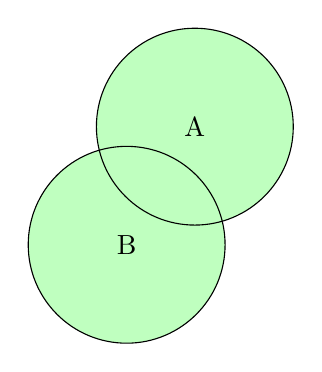
\begin{tikzpicture}
            {
    \def\firstcircle{(90:1cm) circle (1.25cm)}
    \def\secondcircle{(210:1cm) circle (1.25cm)}

    \fill[green!25] \firstcircle;
    \fill[green!25] \secondcircle;

    \draw \firstcircle node {A};
    \draw \secondcircle node {B};
}

        \end{tikzpicture}
        \label{fig:union}
    }
    \subfigure[Durchschnitt $A\cap B$]{
        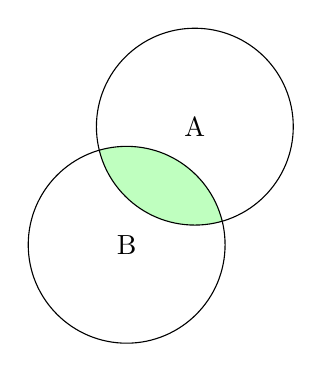
\begin{tikzpicture}
            {
    \def\firstcircle{(90:1cm) circle (1.25cm)}
    \def\secondcircle{(210:1cm) circle (1.25cm)}

    \begin{scope}
        \clip \firstcircle;
        \fill[green!25] \secondcircle;
    \end{scope}

    \draw \firstcircle node {A};
    \draw \secondcircle node {B};
}

        \end{tikzpicture}
        \label{fig:intersection}
    }
    \subfigure[Mengendifferenz $A\setminus B$]{
        \begin{tikzpicture}
            \input{chapters/mathematische_hintergruende/difference}
        \end{tikzpicture}
        \label{fig:difference}
    }
    \subfigure[Symm. Differenz $A\setminus B$]{
        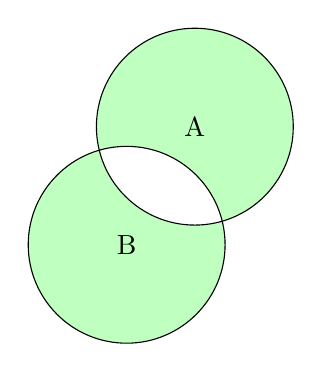
\begin{tikzpicture}
            {
    \def\firstcircle{(90:1cm) circle (1.25cm)}
    \def\secondcircle{(210:1cm) circle (1.25cm)}

    \fill[green!25] \firstcircle;
    \fill[green!25] \secondcircle;

    \begin{scope}
        \clip \firstcircle;
        \fill[white] \secondcircle;
    \end{scope}

    \draw \firstcircle node {A};
    \draw \secondcircle node {B};
}

        \end{tikzpicture}
        \label{fig:symmetric_difference}
    }

    \label{fig:set}
    \caption{Die einzelnen Mengenoperationen}
\end{figure}

\section{Logarithmus-Rechenregeln}\index{Logarithmus-Rechenregeln}\label{sec:logarithmus}
\subsection{Produkte}\index{Logarithmus-Rechenregeln!Produkte}\label{sec:logarithmus_produkte}
\[\log_b(x\cdot y)=\log_b(x)+\log_b(y)\;\;\Rightarrow\;\;\log _{b}\prod _{{i=1}}^{n}x_{i}=\sum _{{i=1}}^{n}\log _{b}x_{i}\]

\subsection{Quotienten}\index{Logarithmus-Rechenregeln!Quotienten}
\[\log_b\left(\frac{x}{y}\right)=\log_b(x)-\log_b(y)\]

\subsection{Potenzen}\index{Logarithmus-Rechenregeln!Potenzen}
\[\log_b \left(x^r\right)=r\cdot \log_b(x)\]

\subsection{Basisumrechnung}\index{Logarithmus-Rechenregeln!Basisumrechnung}
\[\log_b x=\frac{\log_a x}{\log_a b}\]

\section{Ungleichungen}\index{Ungleichungen}
\subsection{Umkehrbarkeit}\index{Ungleichungen!Umkehrbarkeit}
\[({T_{1}}\leq {}{T_{2}})\Leftrightarrow ({T_{2}}\geq {}{T_{1}})\]

\subsection{Addition+Subtraktion}\index{Ungleichungen!Addition/Subtraktion}
\[\text{Wenn }T_1<T_2\text{ dann gilt: }T_{1}+T_{3}<T_{2}+T_{3}\]
\[\text{Wenn }T_1<T_2\text{ dann gilt: }T_{1}-T_{3}<T_{2}-T_{3}\]

\subsection{Multiplikation+Division}\index{Ungleichungen!Multiplikation/Division}
\[\text{Aus }T_1<T_2\text{ folgt: }-T_1>-T_2\]
\[\text{Aus }T_1<T_2\text{ folgt: }0<\frac{1}{T_2}<\frac{1}{T_1}\]
\[\text{Aus }T_3>0 \text{ und }T_1<T_2\text{ folgt: }T_1T_3<T_2T_3 \text{ und }\frac{T_1}{T_3}<\frac{T_2}{T_3}\]
\[\text{Aus }T_3<0 \text{ und }T_1<T_2\text{ folgt: }T_1T_3>T_2T_3 \text{ und }\frac{T_1}{T_3}>\frac{T_2}{T_3}\]

\begin{satz}\label{satz:ungleichung}
Bei Punktrechnung mit Zahl $z > 0$ ($z\in\mathbb{R}$) bleiben die Vergleichszeichen erhalten, während sie sich bei Punktrechnung mit Zahl $z<0$ ($z\in\mathbb{R}$) umkehren.
\end{satz}

\subsection{Potenzieren}\index{Ungleichungen!Potenzieren}
\[T_{1}(x)\leq T_{2}(x)\Leftrightarrow \left(T_{1}(x)\right)^{a}\leq \left(T_{2}(x)\right)^{a}\;\;\forall a>0\]
\[T_{1}(x)\leq T_{2}(x)\Leftrightarrow \left(T_{1}(x)\right)^{a}\geq \left(T_{2}(x)\right)^{a}\;\;\forall a<0\]

\section{Differenzengleichungen}\index{Differenzengleichungen}
\subsection{lineare Differenzengleichungen 2.Ordnung}\index{Differenzengleichugen!lineare 2.Ordnung}
Haben die Form:
\[x_{n+2}+ax_{n+1}+bx_n=s_n\;\;\forall n\in\mathbb N\]
Folgende Schritte sind notwendig:
\begin{enumerate}[1)]
\item Bestimmung der allgemeinen Lösung $x_n^{(h)}$ der homogenen Gleichung:\\
    Mit Ansatz $x_n^{(h)}=\lambda^n$ eingesetzt: $\lambda^{n+2}+a\lambda^{n+1}+b\lambda^n=0$ erhält man die charakterisische Gleichung:
    \[\lambda^2+a\lambda+b=0\]

    Löst man diese mit der Quadratischen Lösungsformel muss man 3 Fälle unterscheiden:

    \[
        x_n^{(h)} = \begin{cases} 
                C_1\lambda_1^n+C_2\lambda_2^n &\mbox{falls } \lambda_1 \neq \lambda_2 \mbox{ reell} \\
                r^n(C_1\cos n\varphi+C_2\sin n\varphi) &\mbox{falls } \lambda_{1,2} = r(\cos\varphi\pm i\sin\varphi)\mbox{ konjugiert komplex} \\
                (C_1+C_2n)\lambda_1^n &\mbox{falls } \lambda_1 = \lambda_2 \mbox{ reell} \\
            \end{cases}
    \]

    Die Berechnung der Konstenten $C_1$ bzw. $C_2$ kann nun mit den Anfangsbedingungen erfolgen.

\item Bestimmung der partikulären Lösung $x_n^{(p)}$.
    Sollte $s_n$ nicht $0$ sein, muss man die partikuläre Lösung bestimmen:
    \begin{center}
    \begin{tabular}{|c|c|}
        \hline
        Störfunktion $s_n$ & Versuchslösung $x_n^{(p)}$\\
        \hline
        $1$ & $A$\\
        $r^n$ & $Ar^n$\\
        $\sin(rn)$ oder $\cos(rn)$ & $A\sin(rn)+B\cos(rn)$\\
        $n^k$ (oder Polynom vom Grad $k$) & $A_0+A_1n+A_2n^2+...+A_kn^k$\\
        $n^k\cdot r^k$ & $(A_0+A_1n+A_2n^2+...+A_kn^k)r^n$\\
        \hline
    \end{tabular}
    \end{center}
\item Ermittlung der Lösungsgesamtheit gemäß $x_n=x_n^{(h)}+x_n^{(p)}$
\end{enumerate}

\section{Binomischer Lehrsatz}\index{Binomischer Lehrsatz}\label{sec:binom_lehrsatz}
\[(x+y)^n=\sum_{k=0}^n\binom{n}{k}x^{n-k}y^k\]
\section{Kombinatorik}\index{Kombinatorik}
\subsection{Permutationen(Anordnungen)}\index{Permuationen}\index{Anordnung}
Anordnungen von $n$-Objekten, Reihenfolge wichtig.
\subsubsection{Ohne Wiederholung}
Anordnung von $n$ Objekten, die alle unterscheidbar sind.
Anfangs $n$-Elemente, dann $n-1$, $n-2$, usw. zur Auswahl.
\[n!=n\cdot(n-1)\cdot\cdot\cdot3\cdot2\cdot1\]
\begin{bsp}
Beispielsweise gibt es $4!=4\cdot 3\cdot 2\cdot 1=24$ mögliche Anordnungen von vier verschiedenfarbigen Kugeln in einer Reihe.
\end{bsp}
\subsubsection{Mit Wiederholung}
$i$-tes Objekt $n_i$-fach wiederholt:

Anordnung von $n$ Objekten, manche nicht unterscheidbar. Sind $k$-Objekte ident, sind diese auf den Plätzen vertauschbar, ohne neue Reihenfolge.
\[\frac{n!}{n_1!\cdot n_2!\cdot\cdot\cdot n_k!}\]
\begin{bsp}
Gibt es $\tfrac {4!}{2!\,1!\,1!}={\tfrac {24}{2}}=12$ mögliche Anordnungen von vier 
farbigen Kugeln in einer Reihe, wenn genau zwei der Kugeln die gleiche Farbe 
aufweisen, und ${\tfrac {4!}{2!\,2!}}={\tfrac {24}{4}}=6$ mögliche Anordnungen, 
wenn jeweils zwei Kugeln gleichfarbig sind.
\end{bsp}
\subsection{Kombinationen}\index{Kombinationen}
Auswahlen von $k$ aus $n$ unterscheidbaren Objekten, Reihenfolge unwichtig:
\subsubsection{Ohne Wiederholung}\index{Binomialkoeffizient}\label{sec:binomialkoeffizient}
auch bekannt als \textbf{Binomialkoeffizient}.
\[\binom{n}{k}=\frac{n!}{k!(n-k)!}\]
\begin{bsp}
    \textbf{Lotto!}
    Wenn aus $45$ Zahlen nur $6$ ohne Wiederholung und ohne Beachtung der Reihenfolge ausgewählt werden. 
\end{bsp}
\subsubsection{Mit Wiederholung}
\[\frac{(n+k-1)!}{k!(n-1)!}=\binom{n-1+k}{k}\]
\begin{bsp}
    Aus einer Urne mit fünf nummerierten Kugeln $(n=5)$ wird dreimal eine Kugel gezogen $(k=3)$ und jeweils wieder zurückgelegt. Man kann also bei allen drei Ziehungen immer aus fünf Kugeln auswählen. Wenn man die Reihenfolge der gezogenen Zahlen nicht berücksichtigt, gibt es
    \[\left(\!\!{5 \choose 3}\!\!\right)={\binom {7}{3}}={\frac {7!}{4!\,3!}}=35\]
        verschiedene Kombinationen. 
\end{bsp}
\subsection{Variationen}\index{Variationen}
Auswahlen von $k$ aus $n$ unterscheidbaren Objekten, Reihenfolge ist wichtig.
\subsubsection{Ohne Wiederholung}
Bei einer Variation ohne Wiederholung sollen $k$ von $n$ Objekten (mit $k\leq n$) auf $k$ verfügbare Plätze platziert werden, wobei jedes Objekt nur höchstens einen Platz einnehmen darf.
\[\binom{n}{k}k!=\frac{n!}{(n-k)!}\]
\begin{bsp}
Wenn aus einer Urne mit fünf verschiedenen Kugeln dreimal ohne Zurücklegen gezogen wird, sind $5 \cdot 4 \cdot 3 = 60$ verschiedene Auswahlen möglich: bei der ersten Ziehung noch fünf Möglichkeiten, dann nur noch vier und für die dritte Ziehung schließlich nur noch drei Möglichkeiten.
\end{bsp}
\subsubsection{Mit Wiederholung}
Bei einer Variation mit Wiederholung werden aus $n$ Objekten $k$ Objekte unter Beachtung der Reihenfolge ausgewählt, wobei Objekte auch mehrfach ausgewählt werden können.
\[n^k\]
\begin{bsp}
Wenn aus einer Urne mit fünf verschiedenen Kugeln dreimal mit Zurücklegen gezogen wird, dann sind $5 \cdot 5 \cdot 5 = 5^3 = 125$ verschiedene Auswahlen möglich.
\end{bsp}
